\chapter{Solu��es: Resultados e Discuss�es}
\label{CapSolucoes}

\section{Introdu��o}

\section{Discuss�es Qualitativas, Quantitativas, Efici�ncia e Acur�cia}

\section{Implementa��o Convencional e \textit{Bitstring} com CUDA}

\section{Cases: Discutir as Simula��es no Espa�o Geogr�fico Escolhido.}

\begin{table}[h!]
\centering
\begin{tabular}{c|c|c|c}
  Implementa��o 	& Tempo de Execu��o em CPU (s) 	& Tempo de Execu��o em GPU (s) 	& Speedup		\\ \hline
  Convencional		& $53472$ 			& $6517$ 			& $8.20$ 		\\
  \textit{Bitstring}	& $54795$	 		& $5187$ 			& $10.56$ 		\\
\end{tabular}
\caption{Tempo de execu��o e \textit{speedups} obtidos para as diferentes implementa��es realizadas.}
\label{tab:tempos}
\end{table} 

\begin{figure}[!htb]
  \centering
  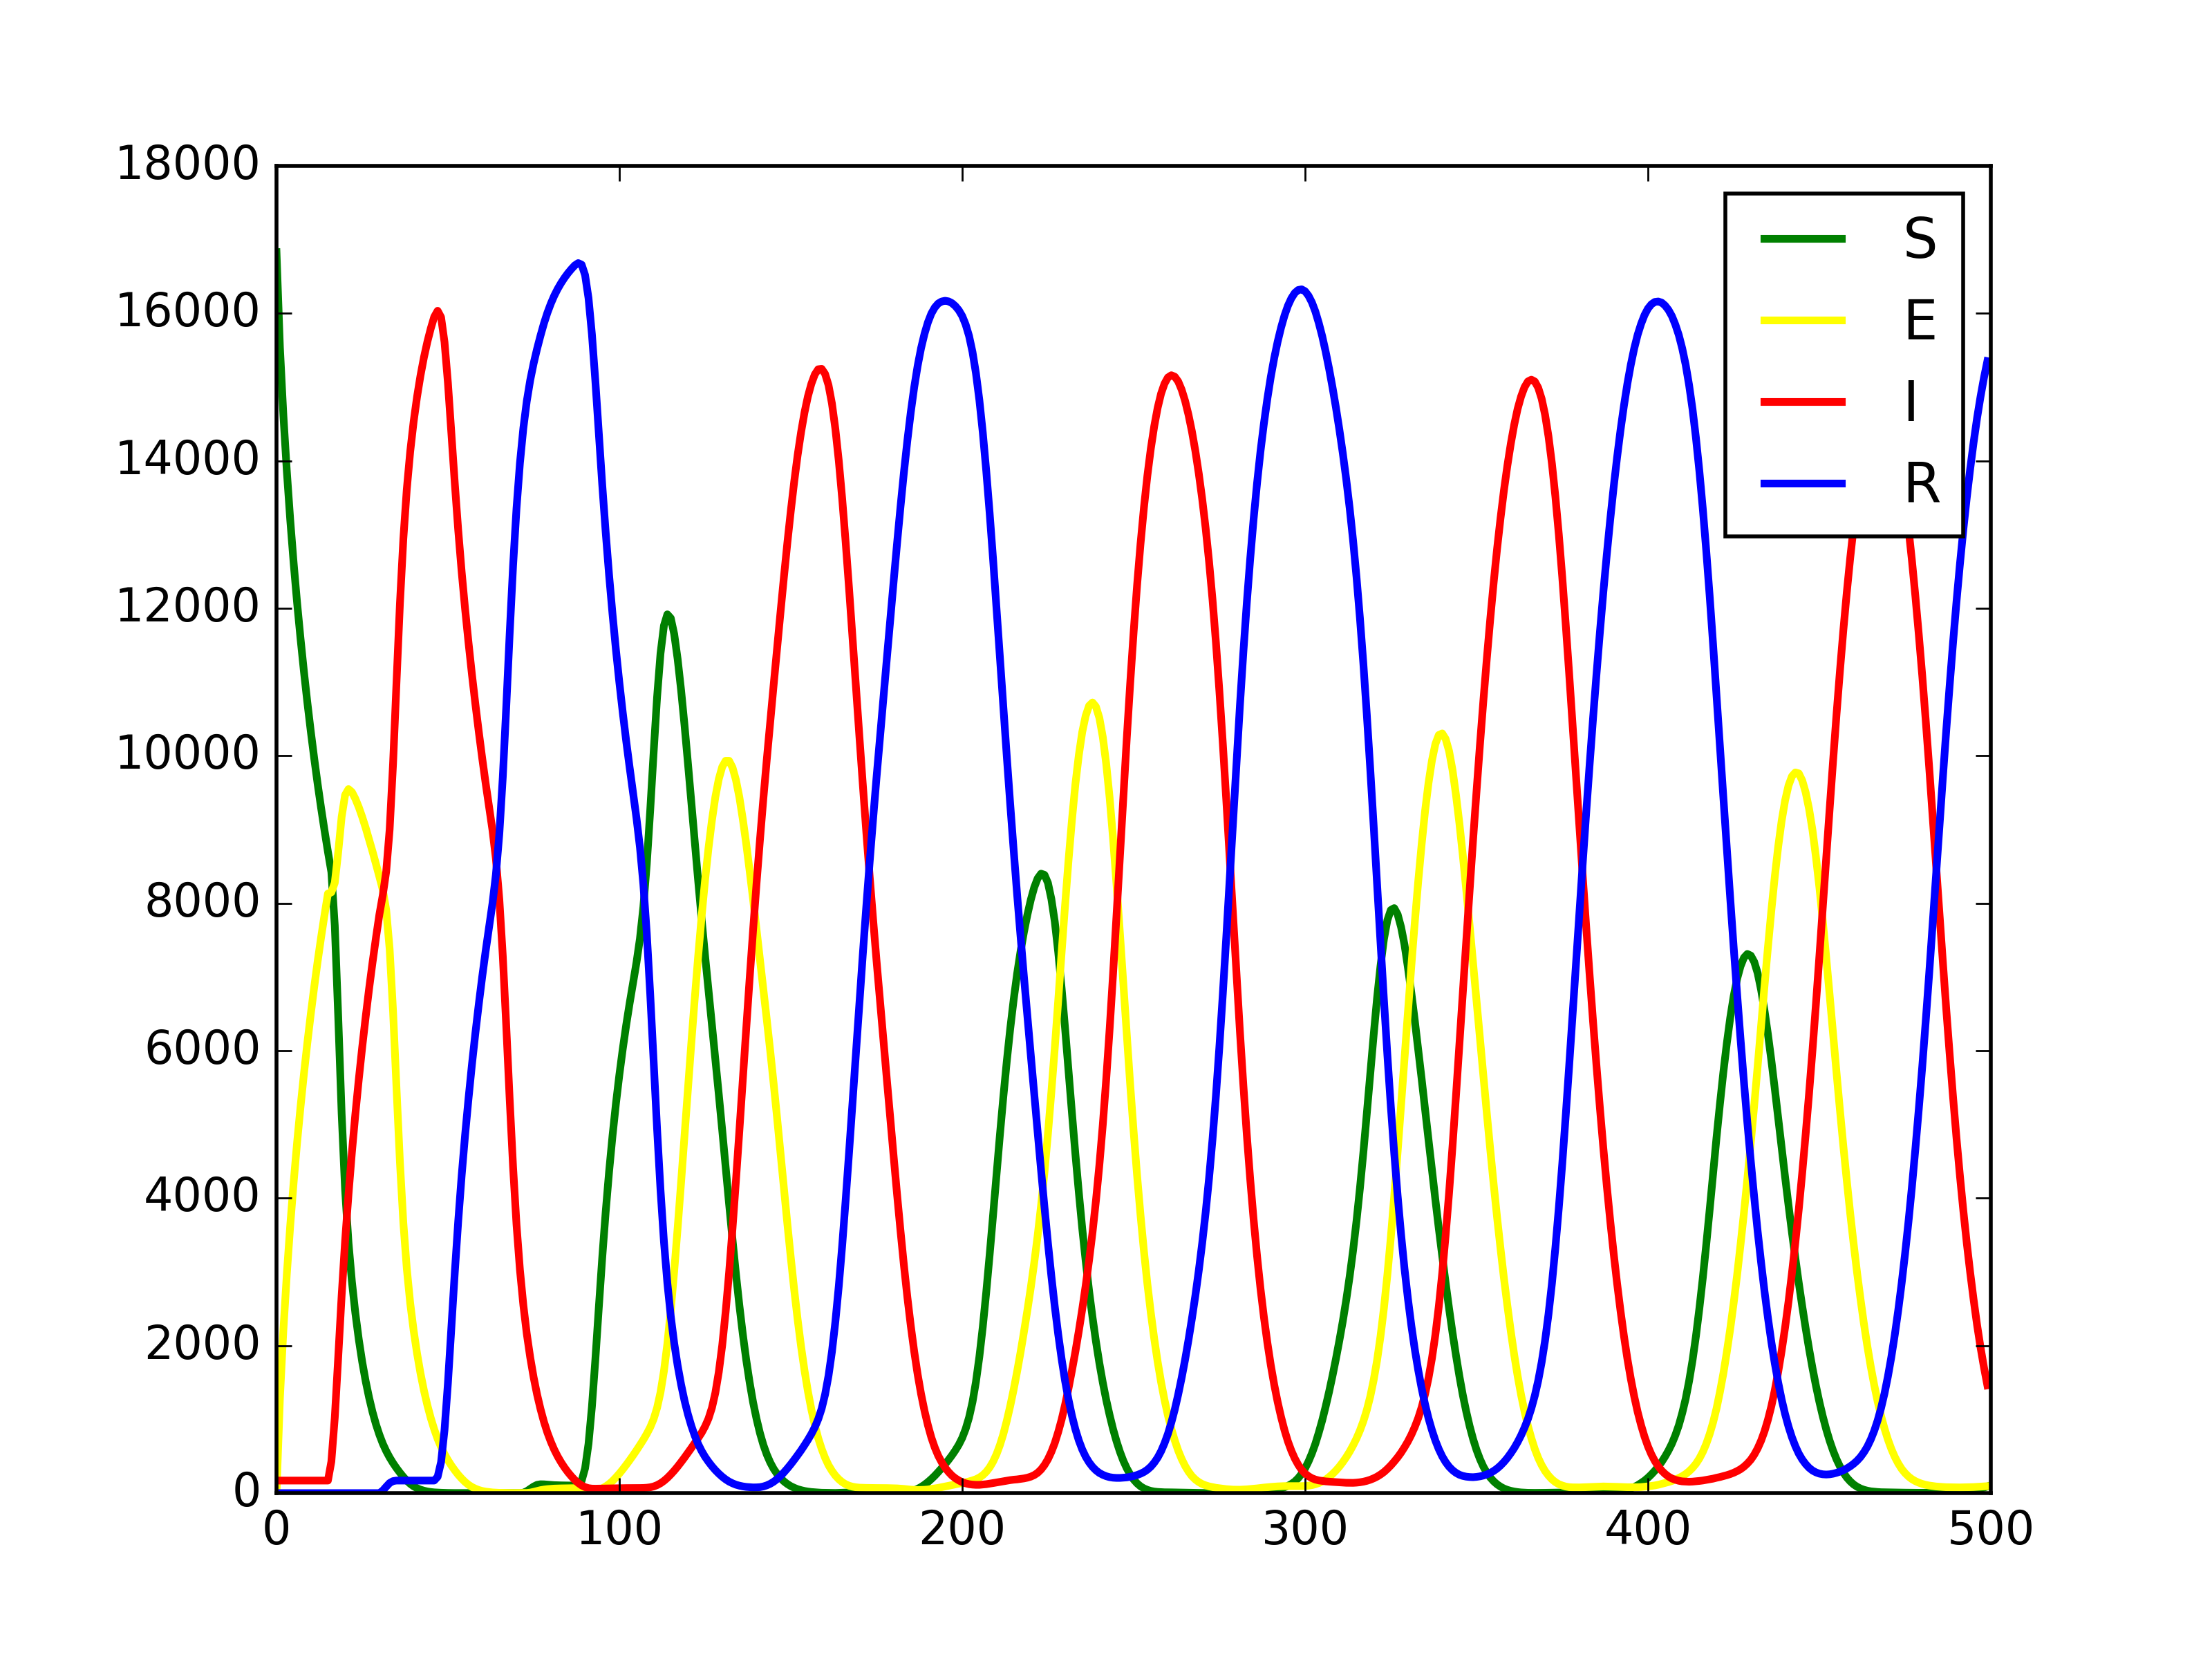
\includegraphics[width=0.8\textwidth]{Figuras/Convencional_CPU.png}
  \caption{Gr�ficos de curvas para a implementa��o convencional em CPU.}
  \label{fig:convencional_cpu}
\end{figure} 

\begin{figure}[!htb]
  \centering
  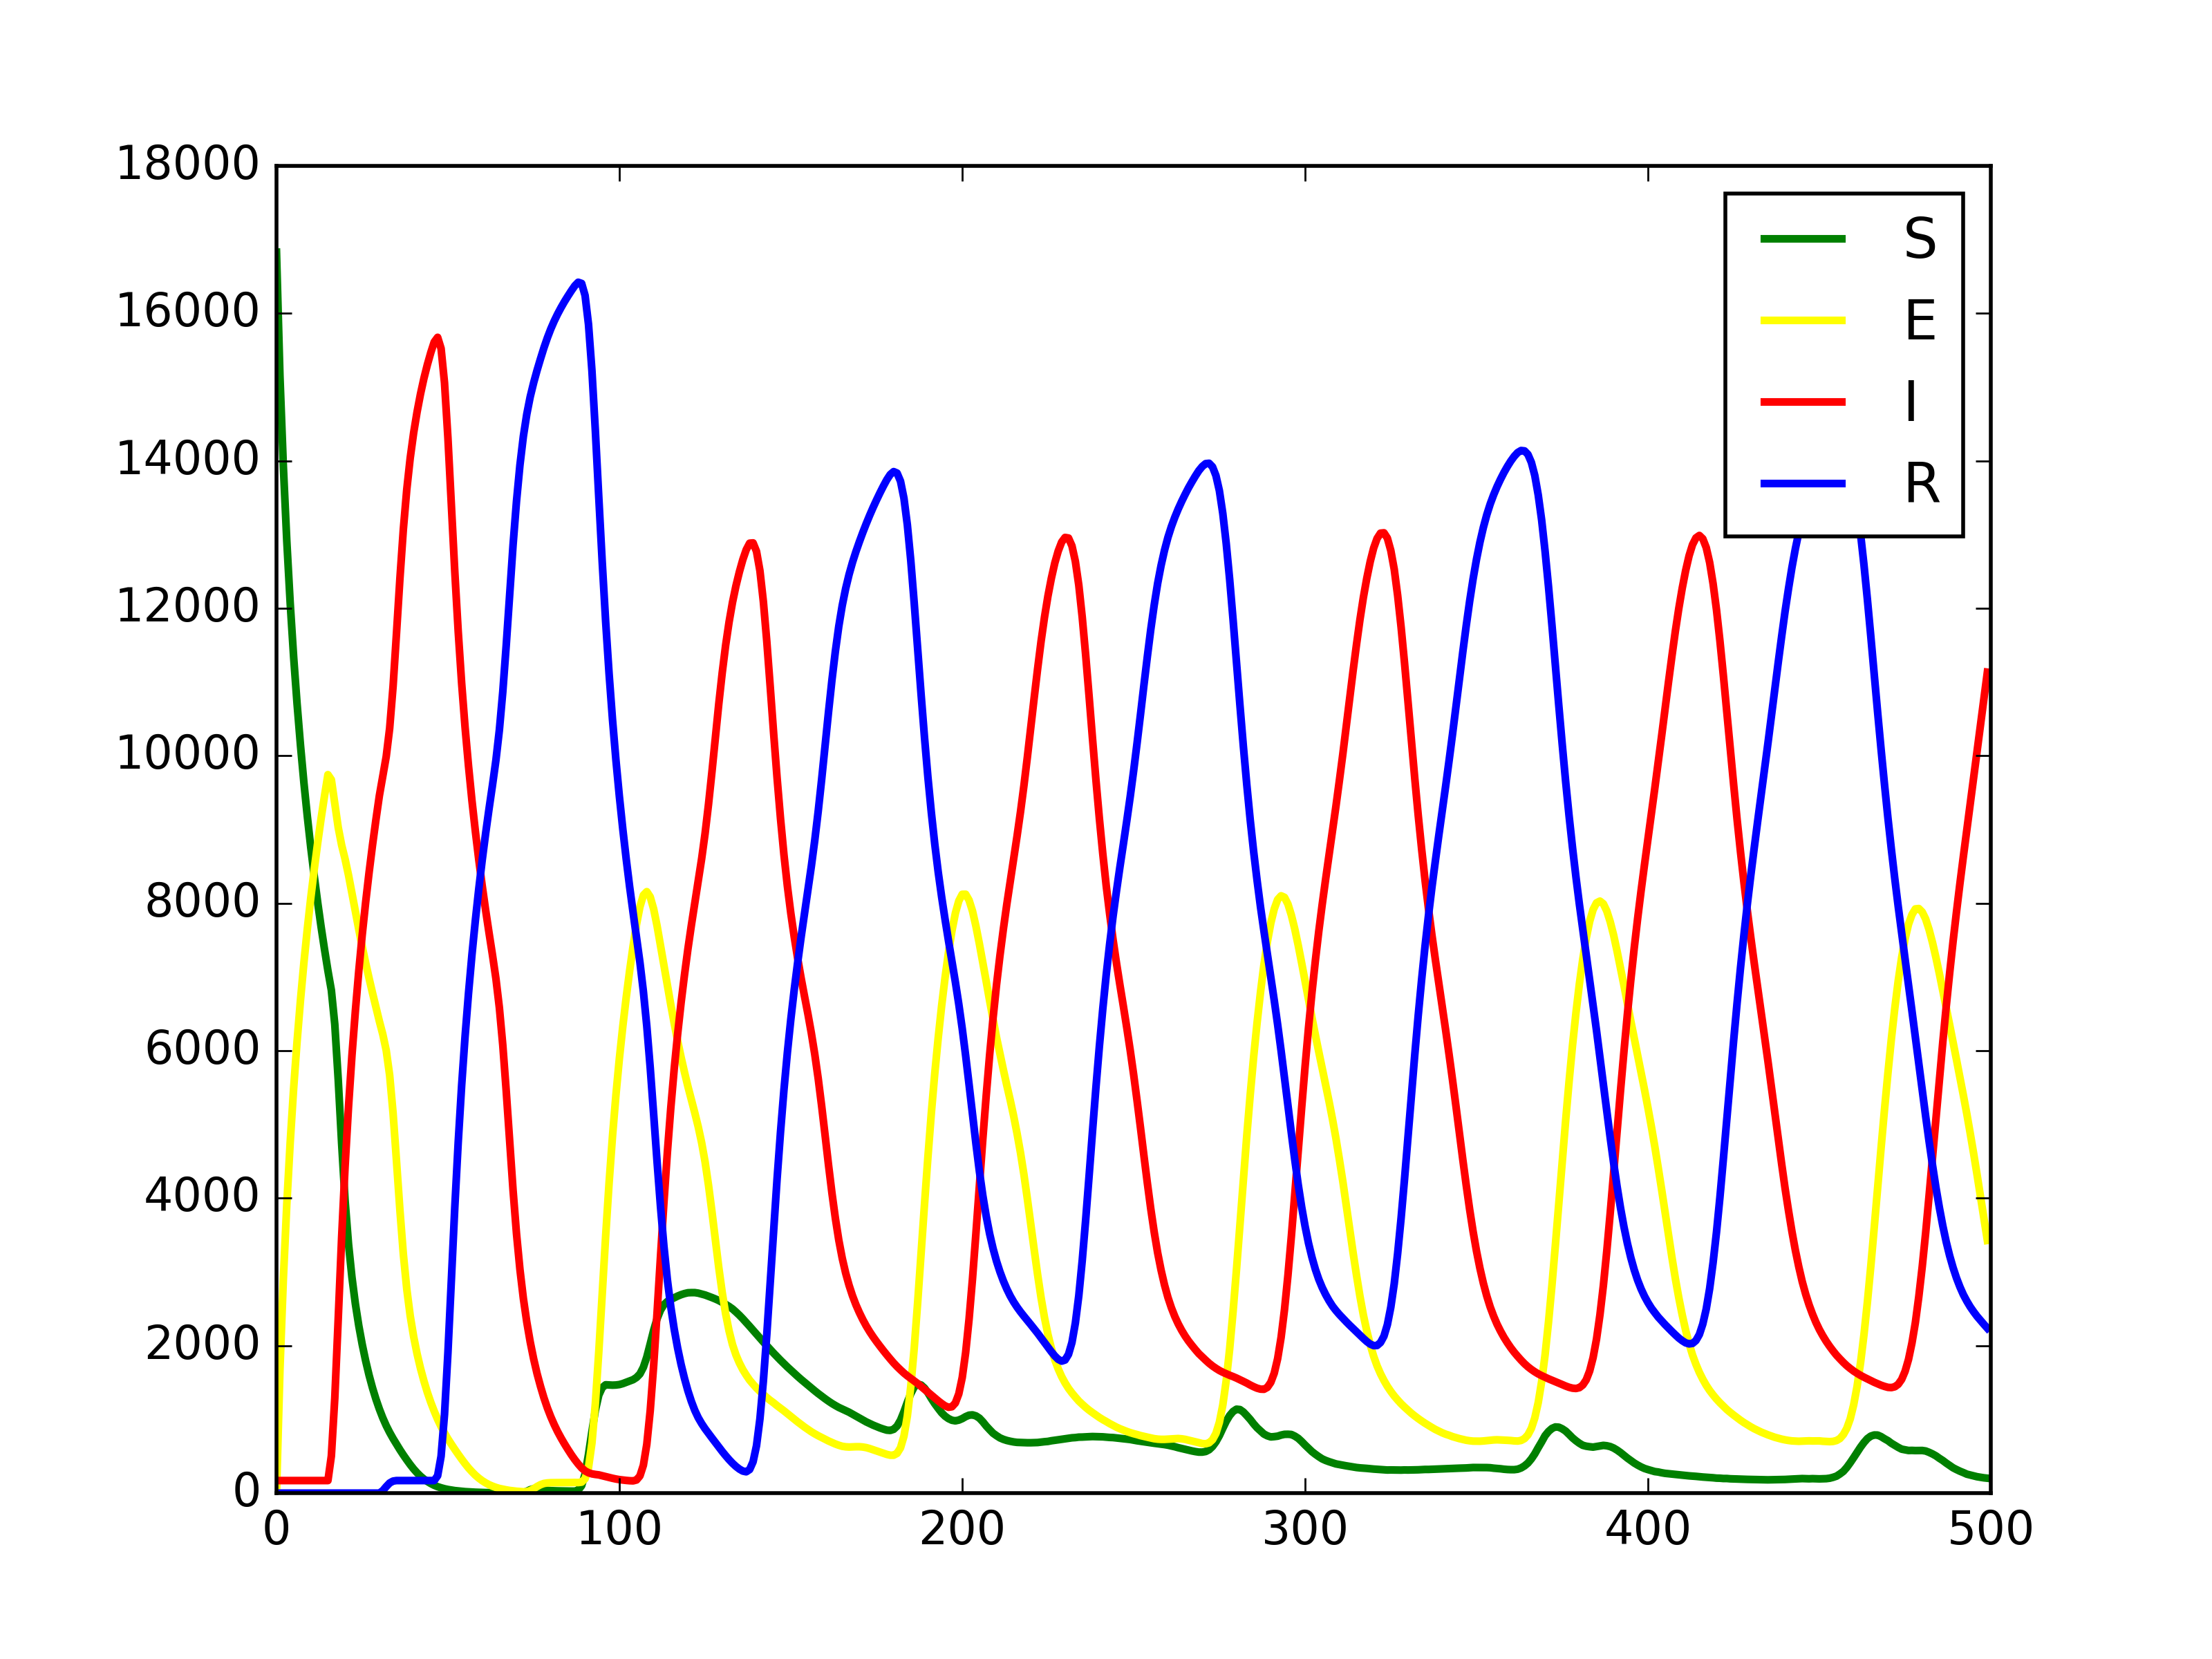
\includegraphics[width=0.8\textwidth]{Figuras/Convencional_GPU.png}
  \caption{Gr�ficos de curvas para a implementa��o convencional em GPU.}
  \label{fig:convencional_gpu}
\end{figure} 

\begin{figure}[!htb]
  \centering
  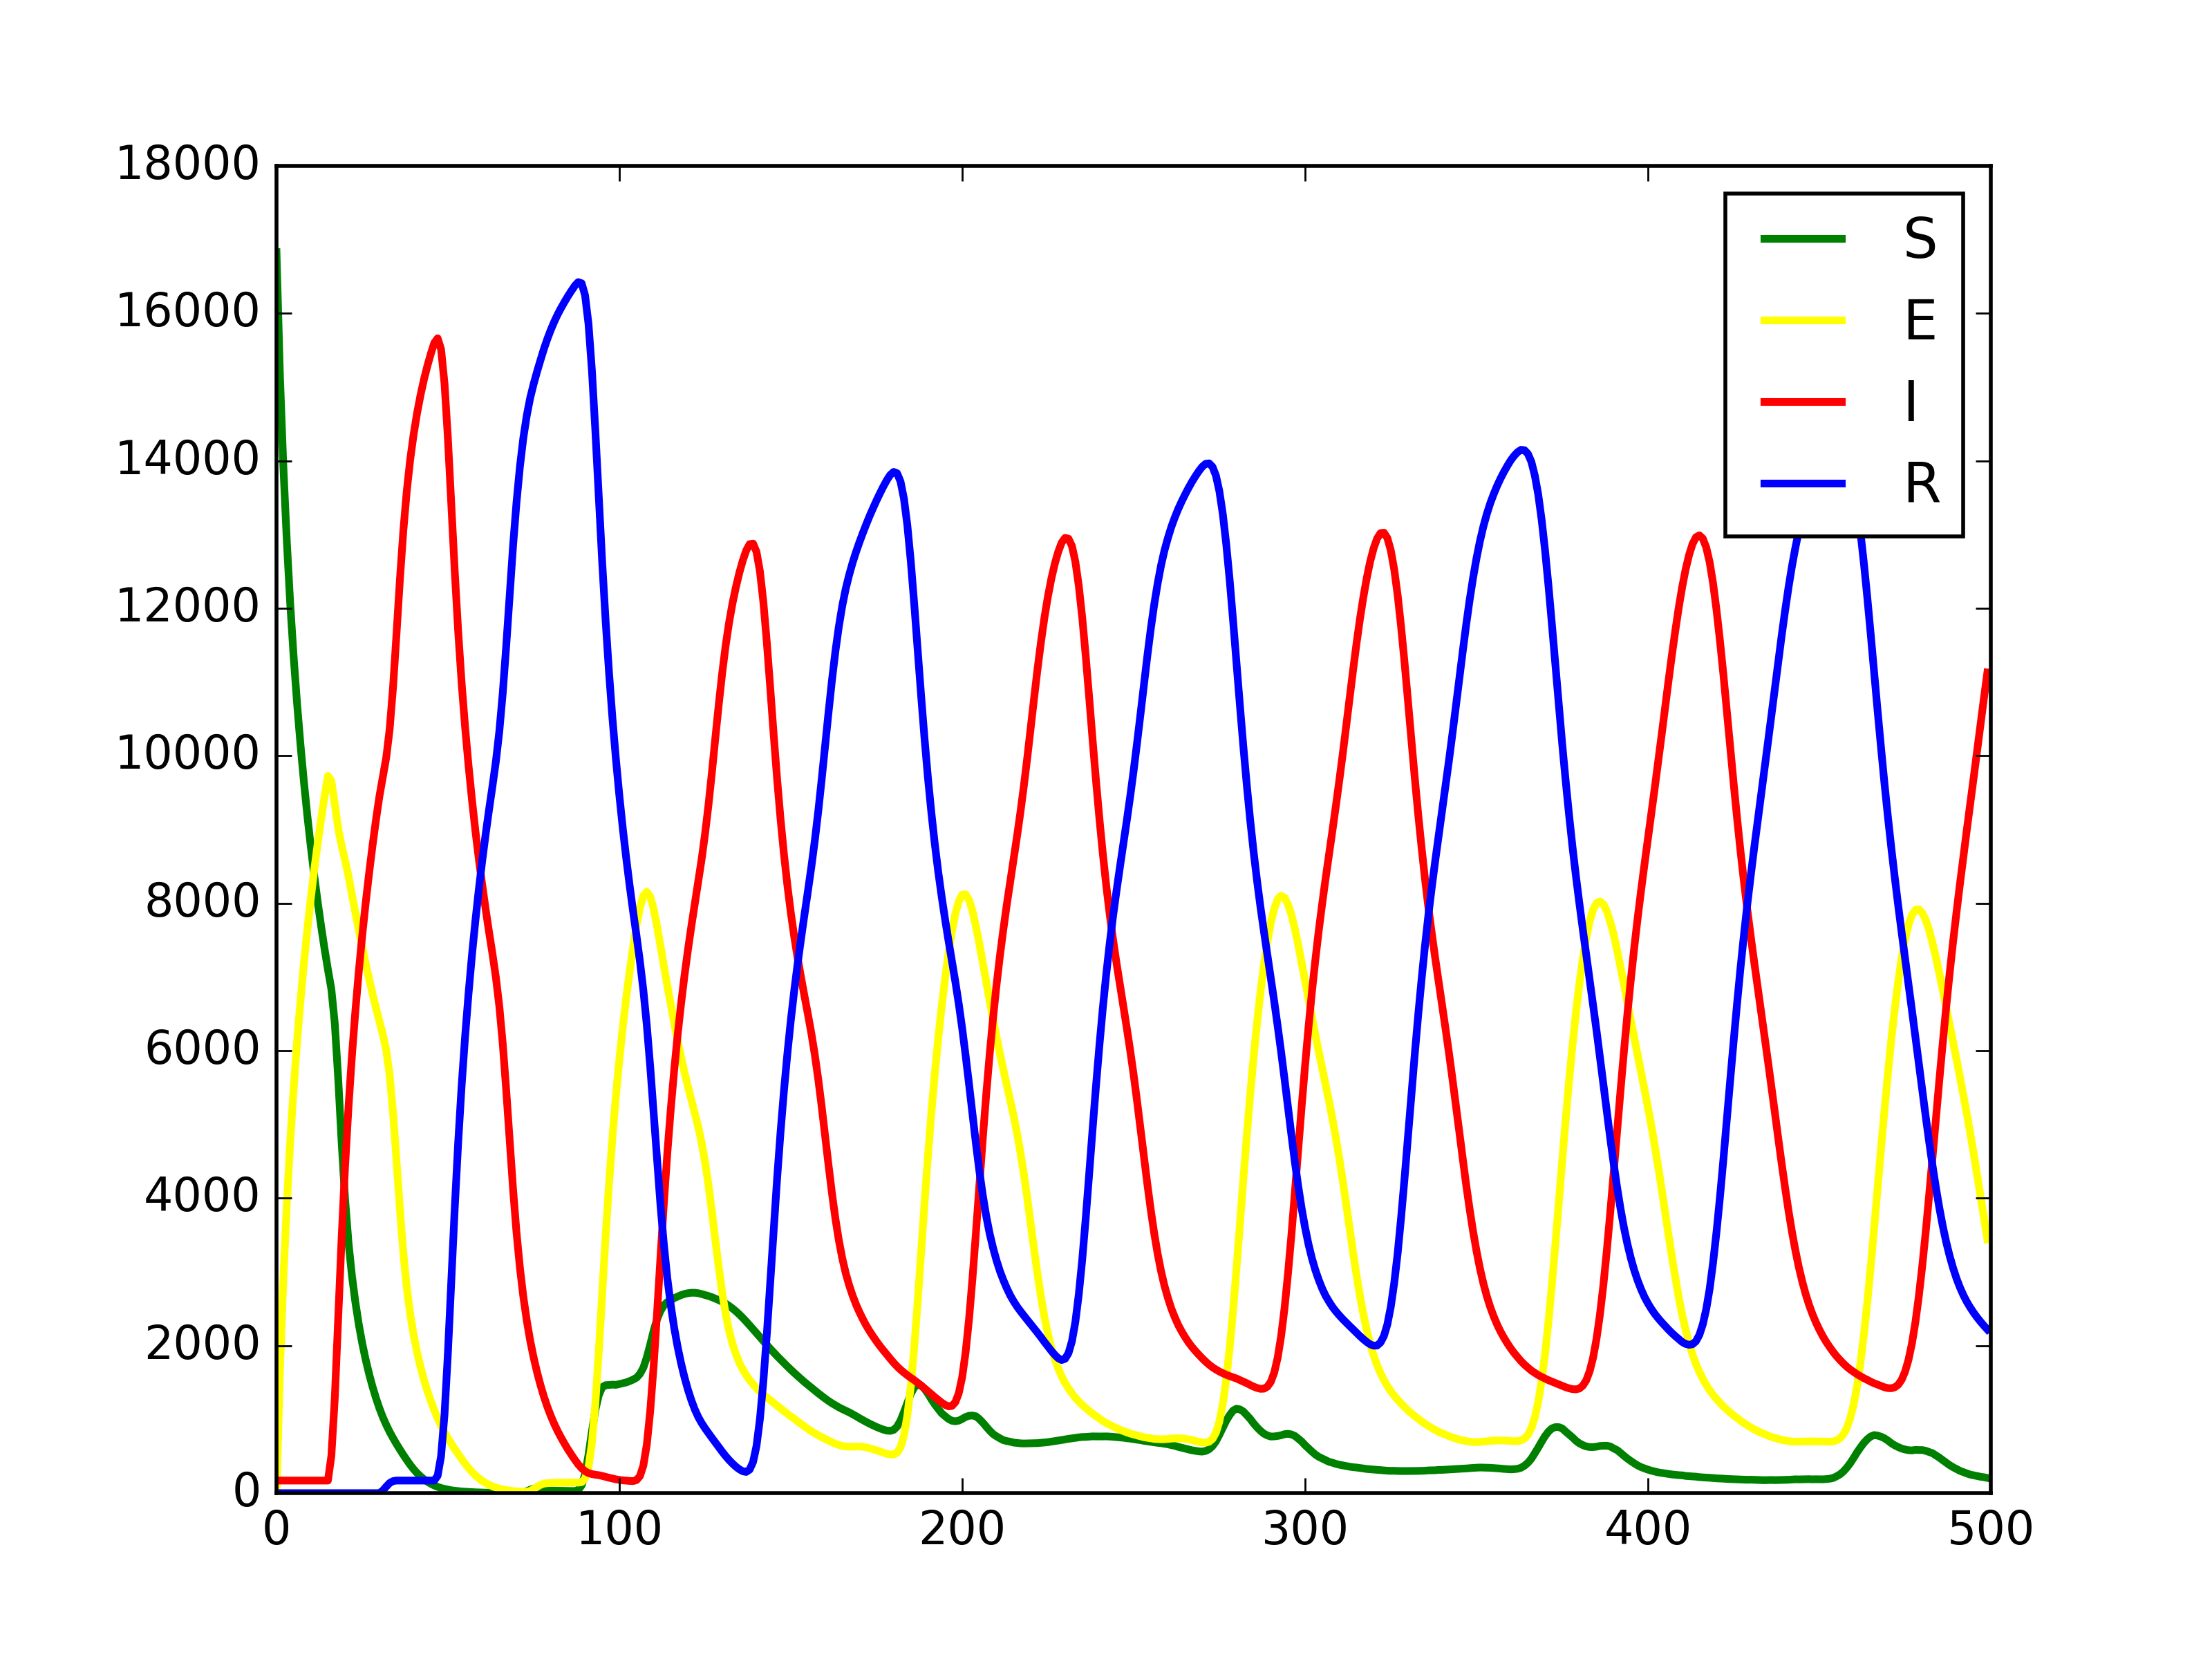
\includegraphics[width=0.8\textwidth]{Figuras/Bitstring_CPU.png}
  \caption{Gr�ficos de curvas para a implementa��o \textit{bitstring} em CPU.}
  \label{fig:bitstring_cpu}
\end{figure} 

\begin{figure}[!htb]
  \centering
  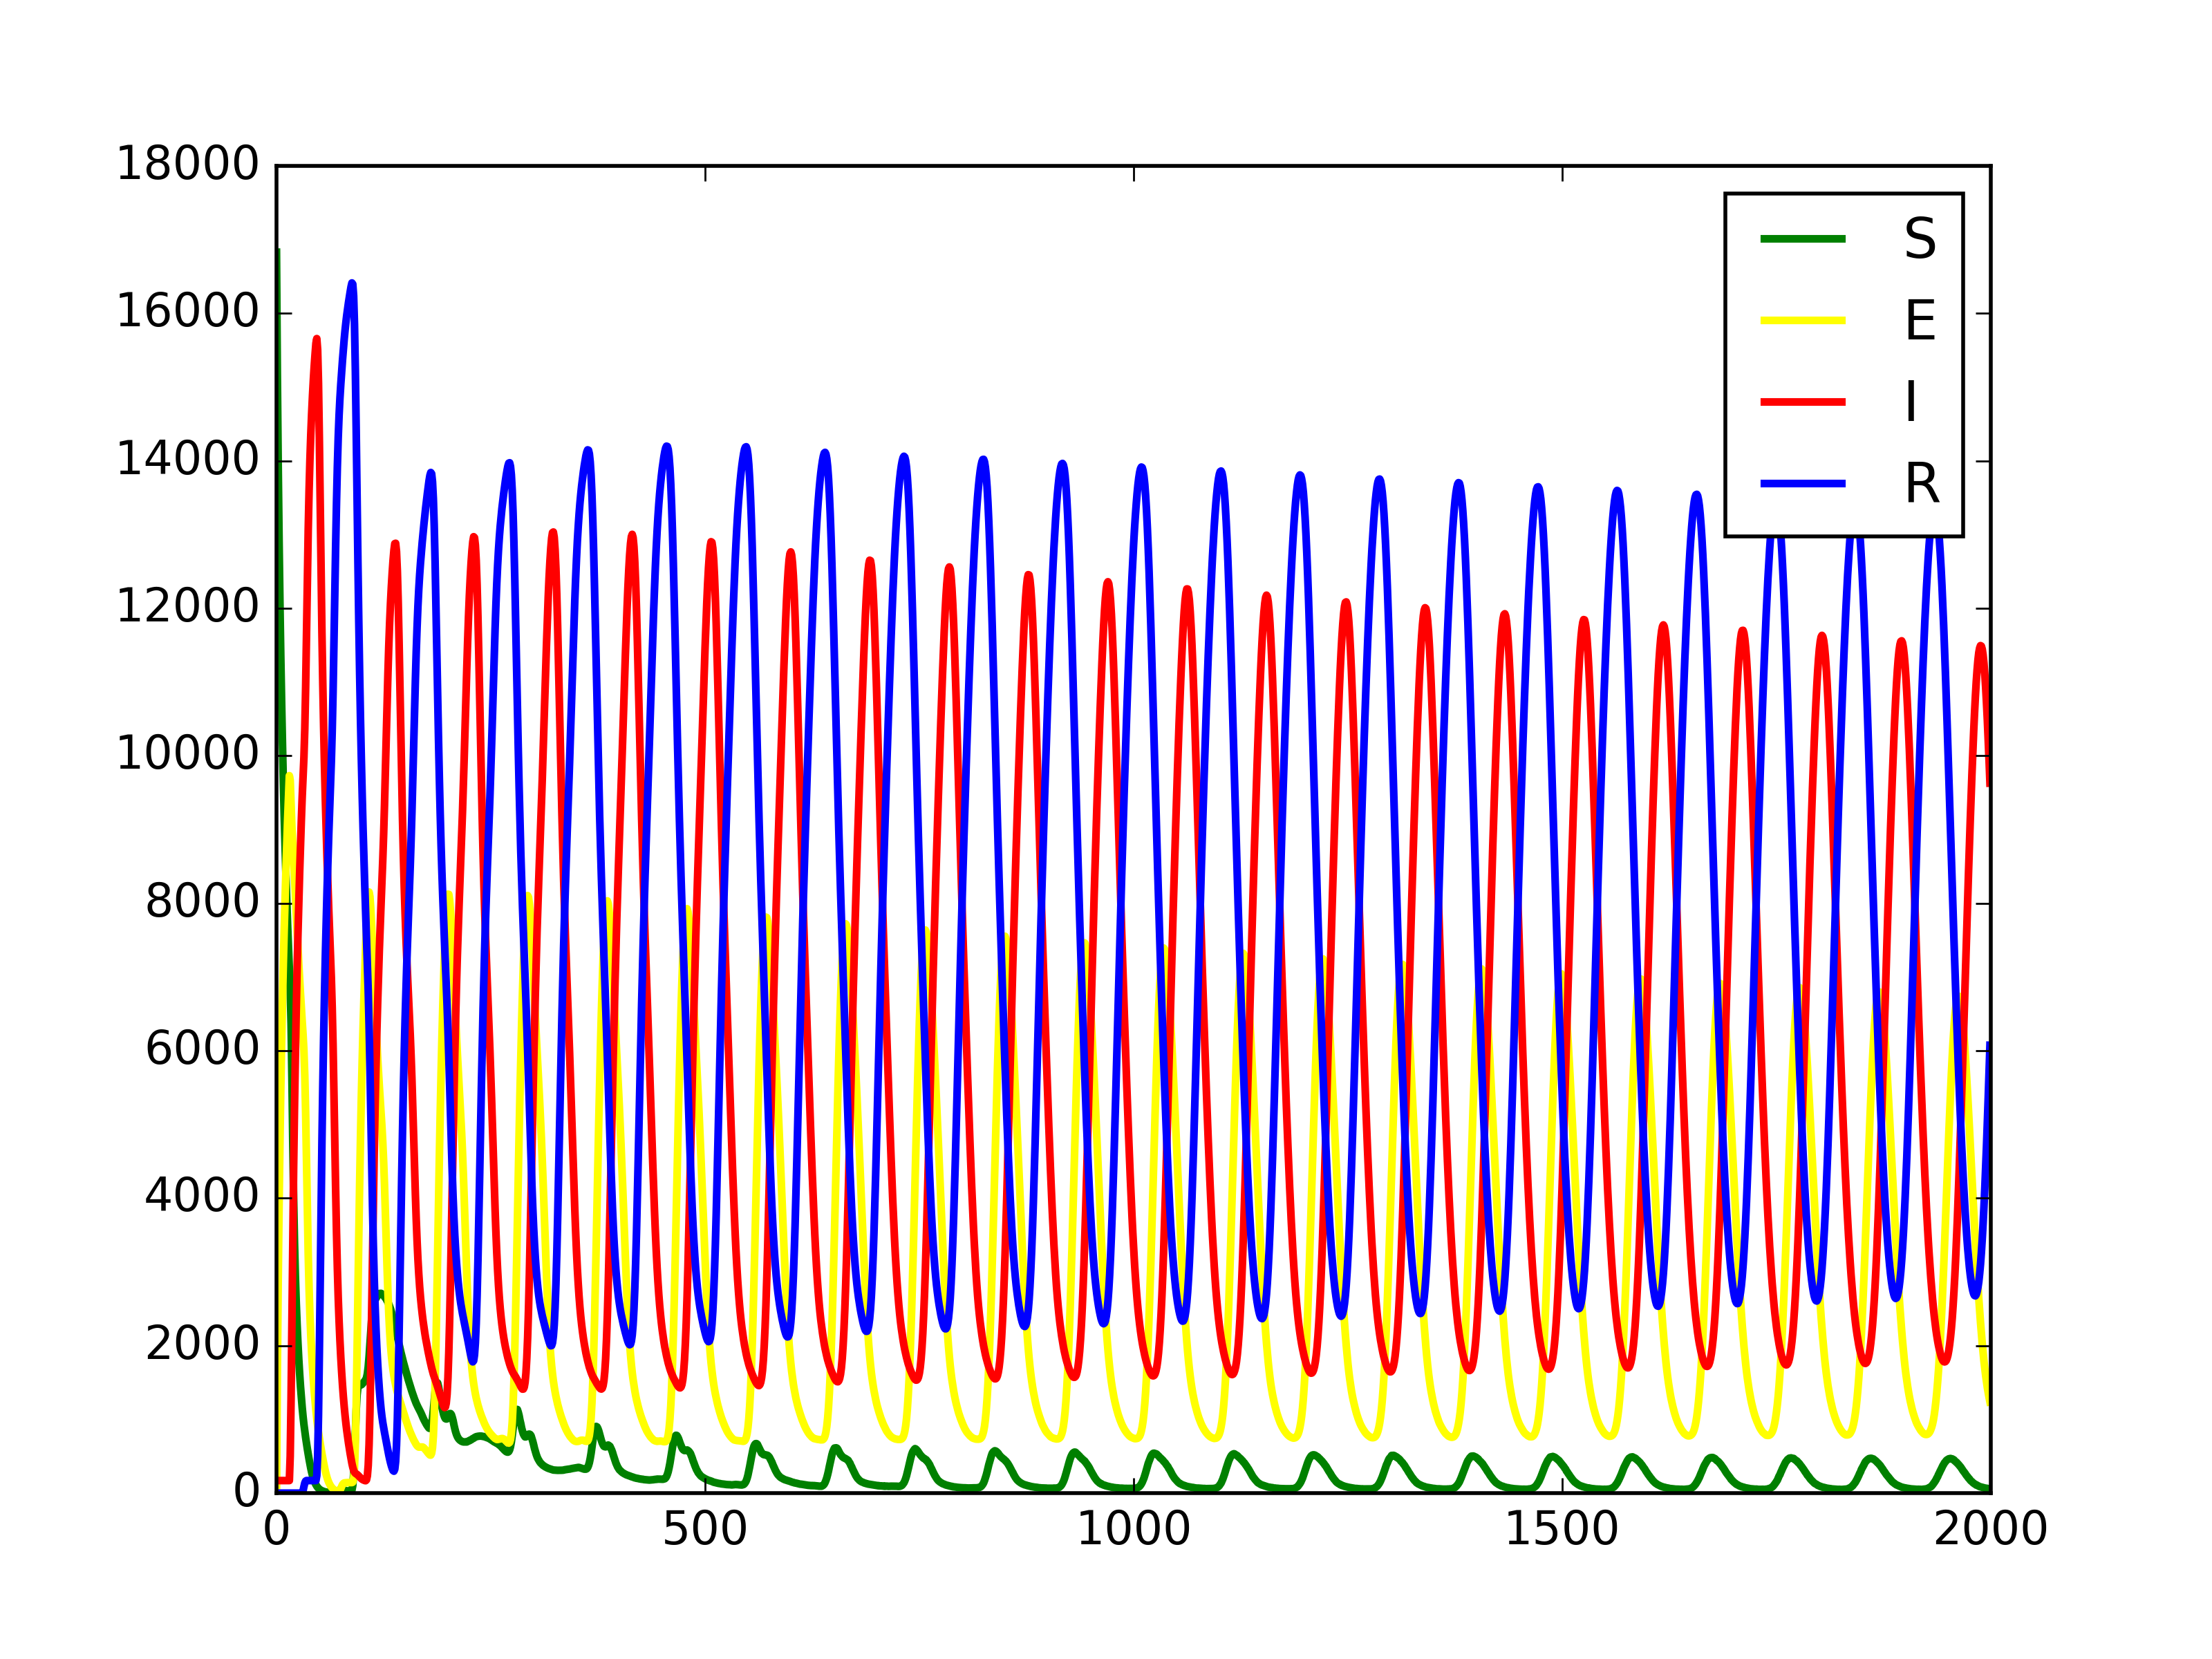
\includegraphics[width=0.8\textwidth]{Figuras/Bitstring_GPU.png}
  \caption{Gr�ficos de curvas para a implementa��o \textit{bitstring} em GPU.}
  \label{fig:bitstring_gpu}
\end{figure} 

\begin{figure}
\centering
\begin{minipage}{.3\textwidth}
  \centering
  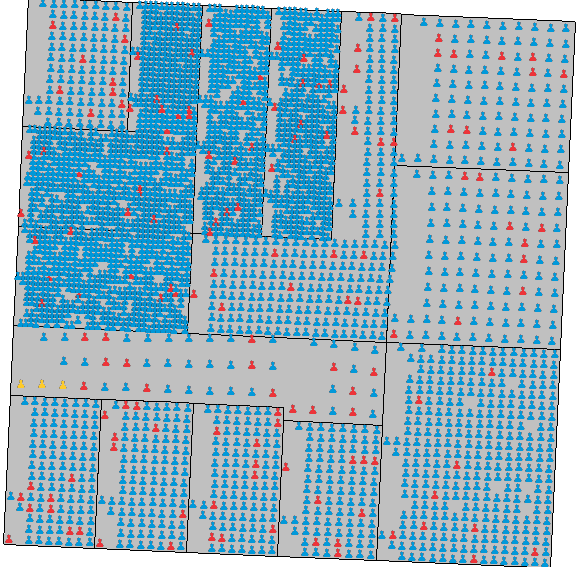
\includegraphics[width=1\linewidth]{Figuras/Convencional/0.png}
  \captionsetup{labelformat=empty}
  \caption*{t = 0.}
\end{minipage}%
\begin{minipage}{.3\textwidth}
  \centering
  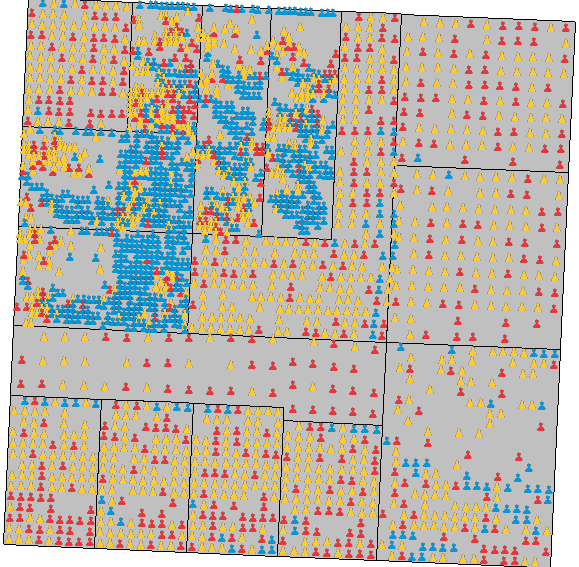
\includegraphics[width=1\linewidth]{Figuras/Convencional/20.png}
  \captionsetup{labelformat=empty}
  \caption*{t = 20.}
\end{minipage}
\begin{minipage}{.3\textwidth}
  \centering
  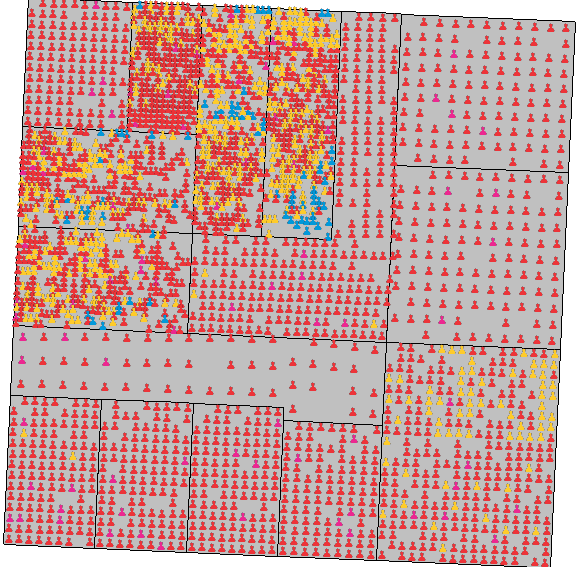
\includegraphics[width=1\linewidth]{Figuras/Convencional/40.png}
  \captionsetup{labelformat=empty}
  \caption*{t = 40.}
\end{minipage}
\begin{minipage}{.3\textwidth}
  \centering
  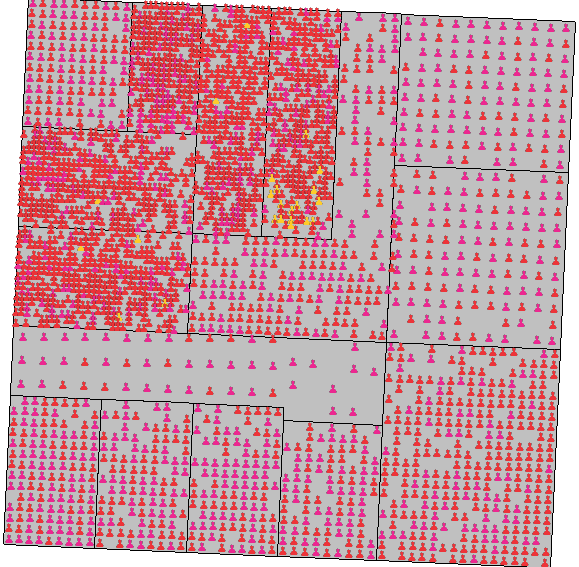
\includegraphics[width=1\linewidth]{Figuras/Convencional/60.png}
  \captionsetup{labelformat=empty}
  \caption*{t = 60.}
\end{minipage}%
\begin{minipage}{.3\textwidth}
  \centering
  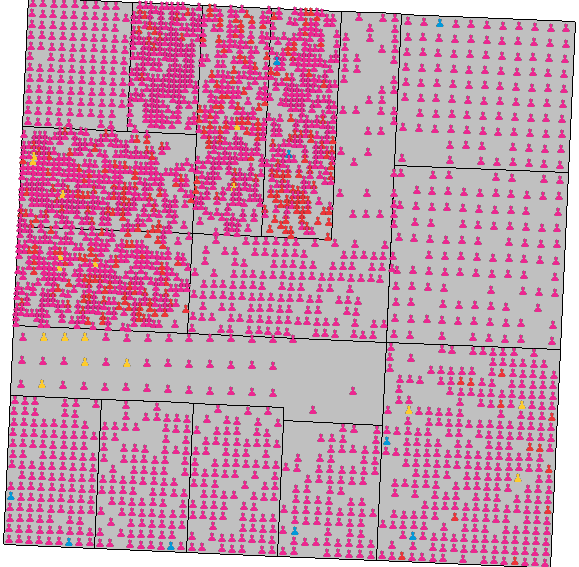
\includegraphics[width=1\linewidth]{Figuras/Convencional/80.png}
  \captionsetup{labelformat=empty}
  \caption*{t = 80.}
\end{minipage}
\begin{minipage}{.3\textwidth}
  \centering
  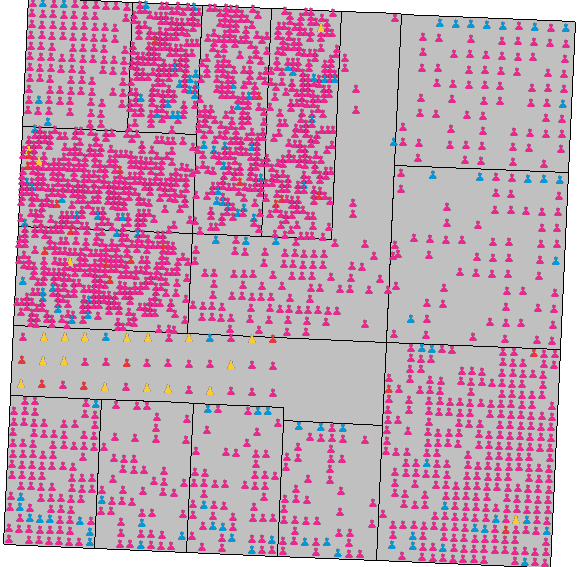
\includegraphics[width=1\linewidth]{Figuras/Convencional/100.png}
  \captionsetup{labelformat=empty}
  \caption*{t = 100.}
\end{minipage}
\caption{Din�mica espa�o-temporal para a implementa��o convencional.}
\end{figure}

\begin{figure}
\centering
\begin{minipage}{.3\textwidth}
  \centering
  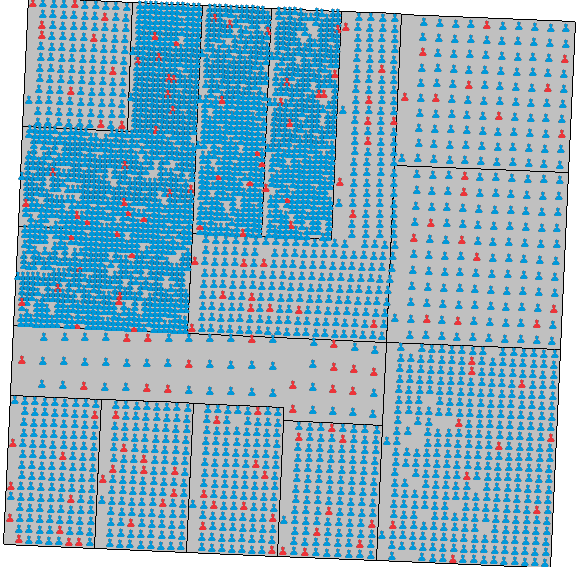
\includegraphics[width=1\linewidth]{Figuras/Bitstring/0.png}
  \captionsetup{labelformat=empty}
  \caption*{t = 0.}
\end{minipage}%
\begin{minipage}{.3\textwidth}
  \centering
  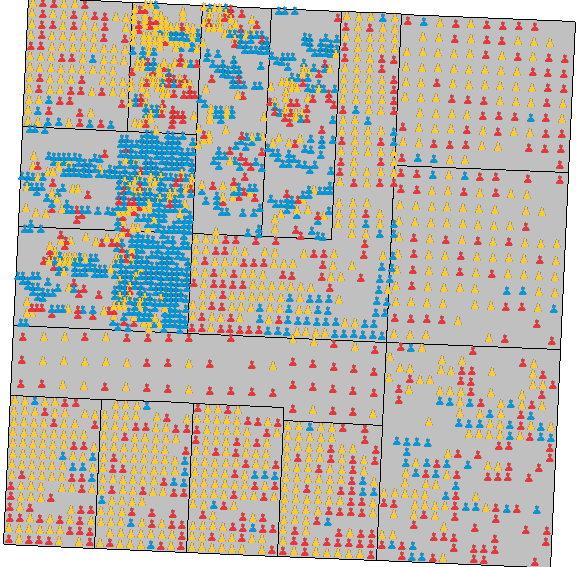
\includegraphics[width=1\linewidth]{Figuras/Bitstring/20.png}
  \captionsetup{labelformat=empty}
  \caption*{t = 20.}
\end{minipage}
\begin{minipage}{.3\textwidth}
  \centering
  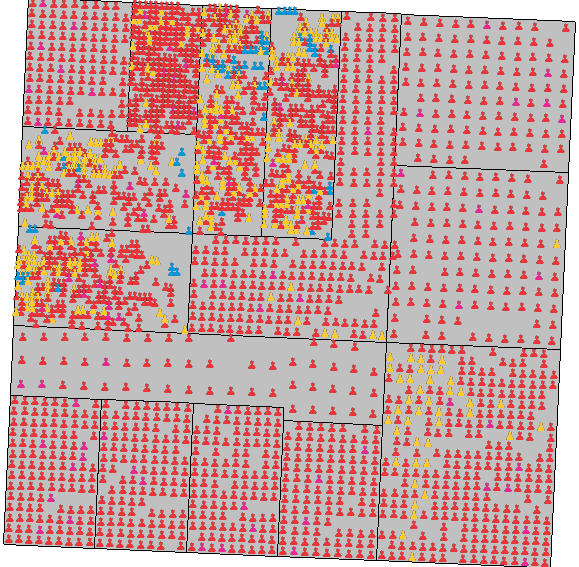
\includegraphics[width=1\linewidth]{Figuras/Bitstring/40.png}
  \captionsetup{labelformat=empty}
  \caption*{t = 40.}
\end{minipage}
\begin{minipage}{.3\textwidth}
  \centering
  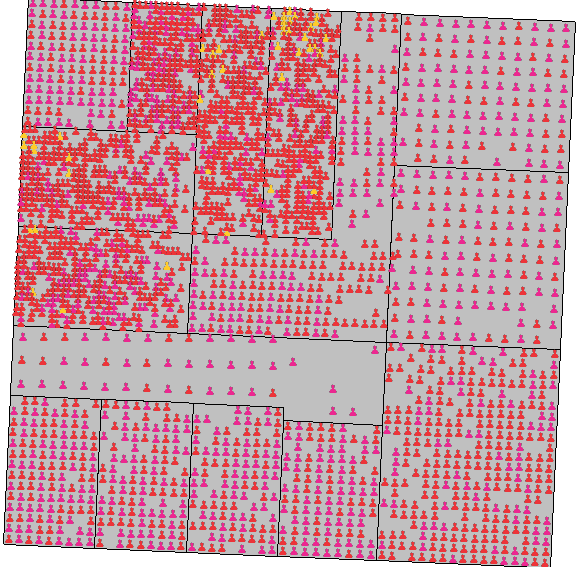
\includegraphics[width=1\linewidth]{Figuras/Bitstring/60.png}
  \captionsetup{labelformat=empty}
  \caption*{t = 60.}
\end{minipage}%
\begin{minipage}{.3\textwidth}
  \centering
  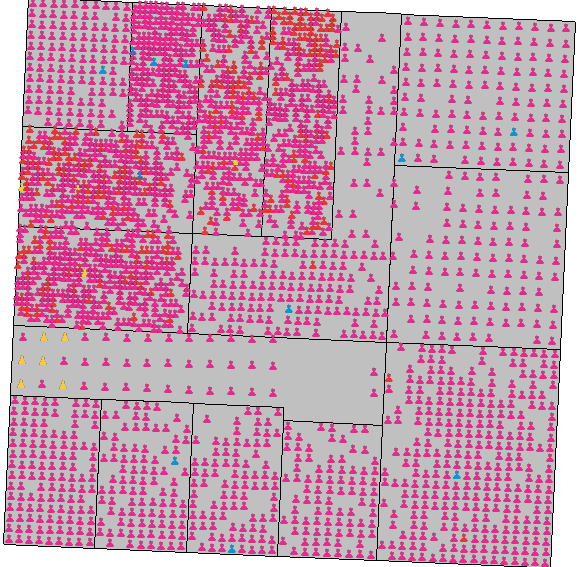
\includegraphics[width=1\linewidth]{Figuras/Bitstring/80.png}
  \captionsetup{labelformat=empty}
  \caption*{t = 80.}
\end{minipage}
\begin{minipage}{.3\textwidth}
  \centering
  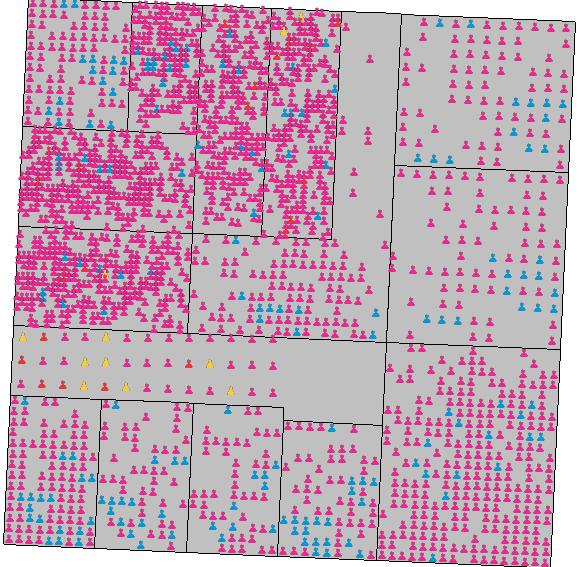
\includegraphics[width=1\linewidth]{Figuras/Bitstring/100.png}
  \captionsetup{labelformat=empty}
  \caption*{t = 100.}
\end{minipage}
\caption{Din�mica espa�o-temporal para a implementa��o \textit{bitstring}.}
\end{figure}
